\section{Quantum Information}


\begin{frame}
\begin{refsection}
	
\vfill

\vspace{-.5cm}\textbf{\Large A Knowledge Compilation Map for Quantum Information}~\cite{qkcm}\vspace{-.5cm}

\vfill

\printbibliography[section=\therefsection]
\end{refsection}

\end{frame}


\begin{frame}{Comparing Decision Diagrams vs RBM vs MPS}

\vspace{-.5em}
\centering

%\begin{figure}[b] 
~\begin{tikzpicture}[-{>[scale=0.3]},>=stealth',shorten >=1pt,auto,node distance=.4cm,
    thick, state/.style={circle,draw,minimum size=10pt,inner sep=.6pt},font=\scriptsize]

\node (vec) {
    \begin{minipage}{1.3cm}\footnotesize
$\def\arraystretch{1.}
    \begin{bmatrix*}[c]
    \frac1{\sqrt 2} \\ 0 \\ 0 \\ 0 \\ 0 \\ 0 \\ 0 \\ \frac1{\sqrt 2}
    \end{bmatrix*}
    $
    \end{minipage}
};


\node[state, right = 2cm of vec.north,anchor=north,yshift=-.2cm] (n1) {$x_3$};

\node[state](n2)[below = of n1, xshift=-.9cm]{$x_2$};
\node[state](n3)[below = of n1, xshift= .9cm]{$x_2$};

\node[state](n21)[below = of n2, ]{$x_1$};
\node[state](n22)[below = of n2, xshift= .9cm]{$x_1$};

\node[state](n31)[below = of n3]{$x_1$};

\node[draw, rectangle,minimum size=.5cm,below = of n21, xshift=.2cm,minimum size=10pt,inner sep=1pt] (l1) {$0$};
\node[draw, rectangle,minimum size=.5cm,right = of l1,minimum size=10pt,inner sep=1pt] (l2) {$\nicefrac1{\sqrt 2}$};


\path[]
(n1) edge[e1] node[right,pos=.7] {} (n3)
(n1) edge[e0] node[left,pos=.7] {} (n2)
(n2) edge[e0] node[left,pos=.7] {} (n21)
(n2) edge[e1] node[left,pos=.7] {} (n22)
(n3) edge[e0] node[left,pos=.7] {} (n22)
(n3) edge[e1] node[left,pos=.7] {} (n31)
(n21) edge[e0=  0]  node[pos=.7] {} (l2)
(n21) edge[e1=  0]  node[pos=.7] {} (l1)
(n22) edge[e0= 20]  node[pos=.7] {} (l1)
(n22) edge[e1= 20]  node[pos=.7] {} (l1)
(n31) edge[e0=  0]  node[pos=.7] {} (l1)
(n31) edge[e1=  0]  node[pos=.7] {} (l2)
;

\node[above=.5cm of n1,anchor=north]    (add) {\textbf{\add}};
\node[left =1.3cm of add]    (svc) {\textbf{Vector}};


\node[state, right=2cm of n1] (q1) {$x_3$} ;
\node[state, below=of q1,xshift=-0.5cm] (q2) {$x_2$} ;
\node[state, below=of q1,xshift=0.5cm] (q3) {$x_2$} ;
\node[state, below=of q2] (q4) {$x_1$} ;
\node[state, below=of q3] (q5) {$x_1$} ;
\node[draw, rectangle,minimum size=.5cm,below = of q4,xshift=0.5cm,minimum size=10pt,inner sep=1pt] (l1) {$1$};


\draw[e0] (q1) edge  node[] {} (q2);
\draw[e1] (q1) edge  node[] {} (q3);
\draw[e0=25] (q2) edge  node[] {} (q4);
\draw[e1=25] (q2) edge  node[,pos=.45] {$0$} (q4);
\draw[e0=25] (q3) edge  node[] {} (q5);
\draw[e1=25] (q3) edge  node[,xshift=-0.6cm,pos=.45] {$0$} (q5);
\draw[e0=-20] (q4) edge  node[] {} (l1);
\draw[e1=-20] (q4) edge  node[,left=.1cm,pos=.45] {$0$} (l1);
\draw[e0=-20] (q5) edge  node[] {} (l1);
\draw[e1=-20] (q5) edge  node[,xshift=0.4cm,pos=.45] {$0$} (l1);
\draw[<-] (q1) --++(90:.5cm) node[right=.2cm,pos=.7,] {$\nicefrac 1{\sqrt 2}$} node[right,pos=.8] {};

\node[right =1.7cm of add]    (sldd) {\textbf{QMDD}};



    \node[state, right = 1.8cm of q1] (a1) {$x_3$};
    \node[state, below = of a1] (a3) {$x_2$};
    \node[state, below = of a3] (a4) {$x_1$};
    \node[draw,rectangle,minimum size=0.5cm, below= of a4,minimum size=10pt,inner sep=1pt] (w4) {1};


    \draw[<-] (a1) --++(90:.5cm) node[right=.2cm,pos=.7,] {$\nicefrac 1{\sqrt 2} \cdot \id^{\otimes3}$} node[left,pos=.8] {};
    \draw[e0=25] (a1) edge  node[] {} (a3);
    \draw[e1=25] (a1) edge  node[pos=.3,right] {$X \otimes X$} (a3);
    \draw[e0=25] (a1) edge  node[] {} (a3);
    \draw[e1=25] (a3) edge  node[pos=.3,right] {$0$} (a4);
    \draw[e0=25] (a3) edge  node[] {} (a4);
    \draw[e0=25] (a4) edge  node[] {} (w4);
    \draw[e1=25] (a4) edge  node[pos=.3,right] {0} (w4);

\node[right=1.4cm of sldd]    (limdd) {\textbf{\limdd}};


%\pause

\node[state, xshift=-5cm, below=.7cm of l1,yshift=.cm] (h1) {$h_1$} ;
\node[state, right=.65cm of h1] (h2) {$h_2$} ;
\node[state, right=.65cm of h2] (h3) {$h_3$} ;
\node[state, right=.65cm of h3] (h4) {$h_4$} ;
\node[state, below=1.7cm of h1, xshift=0.5cm] (v1) {$v_1$} ;
\node[state, right=.7cm of v1] (v2) {$v_2$} ;
\node[state, right=.7cm of v2] (v3) {$v_3$} ;


\draw[e1] (h1) edge  node[] {} (v1);
\draw[e1=-10] (h1) edge  node[] {} (v2);
\draw[e1=-10] (h1) edge  node[] {} (v3);
\draw[e1=10] (h2) edge  node[] {} (v1);
\draw[e1] (h2) edge  node[] {} (v2);
\draw[e1=-10] (h2) edge  node[] {} (v3);
\draw[e1=10] (h3) edge  node[] {} (v1);
\draw[e1] (h3) edge  node[] {} (v2);
\draw[e1=-10] (h3) edge  node[] {} (v3);
\draw[e1=10] (h4) edge  node[] {} (v1);
\draw[e1=10] (h4) edge  node[] {} (v2);
\draw[e1] (h4) edge  node[] {} (v3);


\node[draw,rectangle, below=0.2cm of h1, fill=white, opacity=1] (1) {$i\pi/3$};
\node[draw,rectangle, below=0.2cm of h2, fill=white, opacity=1] (1) {$i\pi/3$};
\node[draw,rectangle, below=0.2cm of h3, xshift=-0.2cm, fill=white, opacity=1] (1) {$-i\pi/3$};
\node[draw,rectangle, below=0.2cm of h4, fill=white, opacity=1] (1) {$-i\pi/3$};


\node[above=0.cm of h3,xshift=-0.6cm]    (a31) {{hidden layer}};
\node[below=0.cm of v2,xshift=0.1cm]    (a31) {{visible layer}};

\node[below=.2cm of l1,xshift=-3.3cm]    (rbm) {\textbf{RBM}};



\node[right=.7cm of h4] (a30) {$A_3^0=\begin{bmatrix}1 & 0\end{bmatrix}$};
\node[right=2cm of a30.west, anchor=west]   (a31) {$A_3^1=\begin{bmatrix}0 & 1\end{bmatrix}$};
\node[below=1.cm of a30.west, anchor=west] (a20) {$A_2^0=\begin{bmatrix}1 & 0 \\ 0 & 0\end{bmatrix}$};
\node[below=1.cm of a31.west, anchor=west] (a21) {$A_2^1=\begin{bmatrix}0 & 0 \\ 0 & 1\end{bmatrix}$};
\node[below=1.cm of a20.west, anchor=west] (a10) {$A_1^0=\begin{bmatrix}\frac1{\sqrt 2} \\ 0\end{bmatrix}$};
\node[below=1.cm of a21.west, anchor=west] (a11) {$A_1^1=\begin{bmatrix}0 \\ \frac1{\sqrt 2}\end{bmatrix}$};

\node[right=3.8cm of rbm]    (a31) {\textbf{MPS}};



\end{tikzpicture}

%\caption{The $3$-qubit GHZ state $\nicefrac{1}{\sqrt 2}(\ket{000} + \ket{111})$, displayed using different data structures.
%The unlabelled edges for \add, \qmdd, \limdd have resp. label 1, 1, $\id$.
%In the RBM, the weights of edges incident to $h_1,h_2$ ($h_3, h_4$) are all $i\pi/3$ ($-i\pi/3$); the hidden node biases $(\beta_{h_1}, \beta_{h_2}, \beta_{h_3}, \beta_{h_4}) = i\pi \cdot (1/3, 2/3, -1/3, -2/3)$; the visible node biases $\alpha_{v_1}=\alpha_{v_2}=\alpha_{v_3}=0$.
%}
%\label{fig:ghz-examples}
%\end{figure}

\pause

\begin{block}{Compare Different Representations Analytically}
	\begin{itemize}\vspace{-.5em}
		\item \textbf{Succinctness}: Families of quantum states showing exponential separations
		\item \textbf{Tractability}: Is manipulation of the representation (e.g., applying a gate) efficient
	\end{itemize}\vspace{-.5em}
\end{block}

\end{frame}




\begin{frame}{Matrix Product States}

\begin{definition}[MPS on $n$ qubits]
	An MPS $M$ is a series of $2n$ matrices of the right dimensions.
	\vspace{.5em}
	
	$A_1^0,~~~ A_2^0,~~~ \dots,~~~ A_n^0$\\
	\vspace{.5em}
	$A_1^1,~~~ A_2^1,~~~ \dots,~~~ A_n^1$
	
	\vspace{.5em}

The interpretation $\ket{M}$ is determined as $\braket{\vec x | M} = A_n^{x_n} \cdot  \cdots  \cdot A_2^{x_2}  \cdot A_1^{x_1}$ for $\vec x \in \{0, 1\}^n$.
\end{definition}

\pause

\begin{exampleblock}{MPS}
	\begin{tikzpicture}[-{>[scale=0.3]},>=stealth',shorten >=1pt,auto,node distance=.4cm,
    thick, state/.style={circle,draw,minimum size=10pt,inner sep=.6pt},font=\scriptsize]

\node (vec) {
    \begin{minipage}{1.3cm}\footnotesize
$\def\arraystretch{1.}
    \begin{bmatrix*}[c]
    \frac1{\sqrt 2} \\ 0 \\ 0 \\ 0 \\ 0 \\ 0 \\ 0 \\ \frac1{\sqrt 2}
    \end{bmatrix*}
    $
    \end{minipage}
};


\node[right=.7cm of vec, yshift=1cm] (a30) {$A_3^0=\begin{bmatrix}1 & 0\end{bmatrix}$};
\node[right=2cm of a30.west, anchor=west]   (a31) {$A_3^1=\begin{bmatrix}0 & 1\end{bmatrix}$};
\node[below=1.cm of a30.west, anchor=west] (a20) {$A_2^0=\begin{bmatrix}1 & 0 \\ 0 & 0\end{bmatrix}$};
\node[below=1.cm of a31.west, anchor=west] (a21) {$A_2^1=\begin{bmatrix}0 & 0 \\ 0 & 1\end{bmatrix}$};
\node[below=1.cm of a20.west, anchor=west] (a10) {$A_1^0=\begin{bmatrix}\frac1{\sqrt 2} \\ 0\end{bmatrix}$};
\node[below=1.cm of a21.west, anchor=west] (a11) {$A_1^1=\begin{bmatrix}0 \\ \frac1{\sqrt 2}\end{bmatrix}$};


\end{tikzpicture}

\end{exampleblock}

	
\end{frame}


\begin{frame}{QMDD vs MPS}


\begin{theorem}
MPS is at least as succinct as QMDD.	
\end{theorem}


\pause

\textbf{Proof:} 

\centering
	\begin{tikzpicture}[-{>[scale=0.3]},>=stealth',shorten >=1pt,auto,node distance=.4cm,
    thick, state/.style={circle,draw,minimum size=10pt,inner sep=.6pt},font=\scriptsize]


\node[yshift=1cm] (a30) {$A_3^0=\begin{bmatrix}1 & 0\end{bmatrix}$};
\onslide<+(1)->{
\node[right=2cm of a30.west, anchor=west]   (a31) {$A_3^1=\begin{bmatrix}0 & 1\end{bmatrix}$};
}
\node[below=1.cm of a30.west, anchor=west] (a20) {$A_2^0=\begin{bmatrix}1 & 0 \\ 0 & 0\end{bmatrix}$};
\onslide<.(1)->{
\node[below=1.cm of a31.west, anchor=west] (a21) {$A_2^1=\begin{bmatrix}0 & 0 \\ 0 & 1\end{bmatrix}$};
}
\node[below=1.cm of a20.west, anchor=west] (a10) {$A_1^0=\begin{bmatrix}\frac1{\sqrt 2} \\ 0\end{bmatrix}$};
\onslide<.(1)->{
\node[below=1.cm of a21.west, anchor=west] (a11) {$A_1^1=\begin{bmatrix}0 \\ \frac1{\sqrt 2}\end{bmatrix}$};
}


\node[state, right=2cm of a31] (q1) {$x_3$} ;
\node[state, below=of q1,xshift=-0.5cm] (q2) {$x_2$} ;
\node[state, below=of q1,xshift=0.5cm] (q3) {$x_2$} ;
\node[state, below=of q2] (q4) {$x_1$} ;
\node[state, below=of q3] (q5) {$x_1$} ;
\node[draw, rectangle,minimum size=.5cm,below = of q4,xshift=0.5cm,minimum size=10pt,inner sep=1pt] (l1) {$1$};


\draw[e0] (q1) edge  node[] {} (q2);
\onslide<.(1)->{
\draw[e1] (q1) edge  node[] {} (q3);
}
\draw[e0=25] (q2) edge  node[] {} (q4);
\onslide<.(1)->{
\draw[e1=25] (q2) edge  node[,pos=.45] {$0$} (q4);
}
\draw[e0=25] (q3) edge  node[] {} (q5);
\onslide<.(1)->{
\draw[e1=25] (q3) edge  node[,xshift=-0.6cm,pos=.45] {$0$} (q5);
}
\draw[e0=-30] (q4) edge  node[above ] {$\frac 1{\sqrt 2}$} (l1);
\onslide<.(1)->{
\draw[e1=-20] (q4) edge  node[,left=.1cm,pos=.45] {$0$} (l1);
}
\draw[e0=-40] (q5) edge  node[right] {$0$} (l1);
\onslide<.(1)->{
\draw[e1=-20] (q5) edge  node[above,xshift=0.cm,pos=.45] {$\frac 1{\sqrt 2}$} (l1);
}
\draw[<-] (q1) --++(90:.5cm) node[right=.2cm,pos=.7,] {} node[right,pos=.8] {};

%\node[right =1.7cm of add]    (sldd) {\textbf{QMDD}};

\end{tikzpicture}

	
\end{frame}



\begin{frame}{\limdd vs MPS}


\begin{lemma}
	There is a family of quantum states with polynomial-size \limdd but exponential-size MPS.
\end{lemma}

\vspace{-.5em}

\textbf{Proof:} It is well-known that MPS can be exponentially sized for stabilizer states.


\vspace{.5em}

\pause


\begin{lemma}
	There is a family of quantum states with polynomial-size MPS but exponential-size \limdd.
\end{lemma}


\vspace{-.5em}
\textbf{Proof sketch:} 

Take the state: \vspace{-2.5em}
\begin{align}
\sumstate = \ket{+}^{\otimes n} + \bigotimes_{j=1}^n(\ket 0+e^{i\pi 2^{-j-1}}\ket 1)
\end{align}
MPS: \vspace{-2.5em}
\begin{align*}
	    A^{0}_1 = \begin{bmatrix} 1 & 1\end{bmatrix}, ~~~~  &A^{x_j}_j = \begin{bmatrix} 1 &  0 \\ 0 & 1 \end{bmatrix}, ~~~~~~ &&A^{x_n}_n = \begin{bmatrix} 1 \\ 1\end{bmatrix}&\\
	    A^{x_1}_1 = \begin{bmatrix} 1 & e^{i\pi 2^{-2}}\end{bmatrix}, ~~~~  &A^{x_j}_j = \begin{bmatrix} 1 &  0 \\ 0 & \prod_{j=2}^{n-1}e^{i\pi 2^{-j-1}}\end{bmatrix},  && A^{x_n}_n = \begin{bmatrix} 1 \\ e^{i\pi 2^{-n-1}}&\end{bmatrix},
	\end{align*}	

LIMDD: There is no LIM mapping subfunctions $f_{\vec a}$ 
to each other for different ${\vec a}$
\[
f_{\vec a}(x_1) = 1 + e^{i\pi \sum_{j=2}^n a_j \cdot 2^{-j-1}} \cdot
e^{i\pi \cdot \nicefrac14 x_1 }.
\]

\end{frame}



\begin{frame}{\limdd vs RBM}
\begin{refsection}


\begin{lemma}
	There is a family of quantum states with polynomial-size RBM but exponential-size \limdd.
\end{lemma}

%\textbf{Proof:}
%
%\begin{columns}[T]
%\begin{column}{0.6\textwidth}
%We use the seminal Boolean function $IP:  \vec{x}, \vec{y} \mapsto  \vec{x}^T  \vec{y} \mod 2$ for even $n$, which computes the inner product between the first half of the input with the second half.
%
%~\\
%
%\citeauthor{martens2013representational}~\cite{martens2013representational} shows RBM is exponential for it.
%\end{column}
%\begin{column}{0.3\textwidth}
%\vspace{-3em}
%\scalebox{.5}{
%\begin{tikzpicture}[
%    scale=0.3,
%    every path/.style={>=latex},
%    every node/.style={},
%    inner sep=0pt,
%    minimum size=14pt,
%    line width=1pt,
%    node distance=.3cm,
%    thick,
%    font=\footnotesize
%    ]
%
%    \node[] (root)   {};
%    \node[draw,circle, below =of root, xshift=0cm] (l1) {};
%    \node[draw,circle, below =of l1] (l2) {};
%
%    \node[draw,circle, below =of l1, xshift=1cm] (ma2) {};
%
%    \node[draw,circle, below =of l2] (l3) {};
%    \node[draw,circle, below =of l2, xshift=3cm] (r3) {};
%    \node[draw,circle, below =of l3] (l4) {};
%    \node[draw,circle, below =of r3] (r4) {};
%    \node[draw,circle, below =of l3, xshift=1cm] (ma4) {};
%    \node[draw,circle, below =of l3, xshift=2cm] (mb4) {};
%
%    \node[draw,circle, below =.6cm of l4] (l5) {};
%    \node[draw,circle, below =.6cm of r4] (r5) {};
%
%    \node[draw,circle, below= of l5] (l6) {};
%    \node[draw,circle, below= of r5] (r6) {};
%    \node[draw,circle, below= of l5, xshift=1cm] (ma6) {};
%    \node[draw,circle, below= of l5, xshift=2cm] (mb6) {};
%
%	 \node[left of =l1] 	{$x_1$};
%	 \node[left of =l2] 	{$x_2$};
%	 \node[left of =l3] 	{$x_3$};
%	 \node[left of =l4] 	{$x_4$};
%	 \node[left  =.1cm of l5] 	{$x_{n-1}$};
%	 \node[left of =l6] 	{$x_{n}$};
%
%    \node[draw,circle,rectangle,minimum size=0.4cm, below=of l6] (leaf0) {$0$};
%    \node[draw,circle,rectangle,minimum size=0.4cm, below=of r6] (leaf1) {$\frac{1}{A}$};
%
%    \draw[<-] (l1) --++(90:2cm) node[pos=1.4,right] {};
%
%    \draw[e0=0] (l1) edge  node[] {} (l2);
%    \draw[e1=0] (l1) edge  node[] {} (ma2);
%
%
%    \draw[e0=25] (l2) edge  node {} (l3);
%    \draw[e1=25] (l2) edge  node {} (l3);
%
%
%    \draw[e0=0] (ma2) edge  node {} (l3);
%    \draw[e1=0] (ma2) edge  node {} (r3);
%
%
%    \draw[e0=0] (l3) edge  node {} (l4);
%    \draw[e1=0] (l3) edge  node {} (ma4);
%
%    \draw[e1=0] (r3) edge  node {} (mb4);
%    \draw[e0=0] (r3) edge  node[left] {} (r4);
%
%    \node[ xshift=0.5cm, yshift=.5cm, below= of ma4] (a) {$\pmb{\vdots}$};
%
%    \draw[e0=0] (l5) edge  node {} (l6);
%    \draw[e1=0] (l5) edge  node {} (ma6);
%
%    \draw[e0=0] (r5) edge  node {} (r6);
%    \draw[e1=0] (r5) edge  node {} (mb6);
%
%    \draw[e0=0] (ma6) edge  node {} (leaf0);
%    \draw[e1=0] (ma6) edge  node {} (leaf1);
%
%    \draw[e0=0] (mb6) edge  node {} (leaf1);
%    \draw[e1=0] (mb6) edge  node {} (leaf0);
%
%    \draw[e0=25] (l6) edge  node {} (leaf0);
%    \draw[e1=25] (l6) edge  node {} (leaf0);
%
%    \draw[e1=25] (r6) edge  node {} (leaf1);
%    \draw[e0=25] (r6) edge  node {} (leaf1);
%\end{tikzpicture}
%}
%\end{column}
%\end{columns}

	
%\onslide<+->{


\begin{lemma}
	There is a family of quantum states with polynomial-size \limdd but exponential-size RBM.
\end{lemma}

%We use the $\ket{Sum}$ state again.
%}

%\printbibliography[section=\therefsection]
\end{refsection}
\end{frame}



\begin{refsection}
\begin{frame}{A Knowledge Compilation Map for Quantum Information}

\begin{theorem}[Decision Diagram vs MPS vs RBM~\cite{qkcm}]
\begin{itemize}
%	\item is a generalization of QMDD
%	\item Nodes are merged up to $\gamma \cdot P_1 \otimes \dots \otimes P_n$ with $P_1, \dots, P_n \in \set{\id, X, Y, Z}$
%	\item<2-> All stabilizer states have linear \limdd size
%	\item<3-> Stabilizer (Clifford) circuit simulation is polynomial time in \limdd
%\pause
%\pause
%	\item RBM is quantum neural network
%	\item MPS is a tensor train (linear tensor network)
	\item<+-> \limdd \& MPS are exponentially more succinct than QMDD \& ADD
	\item<+-> \limdd, MPS \& RBM are incomparable
	\item<+-> Some operations become harder on \limdd
\end{itemize}

\centering

\begin{columns}%[onlywidth,T]
	\begin{column}{.35\textwidth}
\phantom{ZZZZ}
\scalebox{.63}{
\hspace{2em}
\begin{tikzpicture}[node distance=.7cm,minimum height=.5cm]
        % nodes
		\node[draw] (mps) 			   {MPS};
		\node[draw, right =2cm of mps, yshift=-2.1cm] (limdd) {\limdd};
%		\node[draw, above =of limdd, yshift=1.5cm] (tn) {TN};
\onslide<2->{
		\node[draw, right =2cm of limdd, yshift=2.1cm] (rbm) {RBM};
}
%		\node[draw, below =2cm of rbm, xshift=0.4cm,text width=1.3cm, align=center] (ss) {Stabilizer States};
		\node[draw, below = 1cm of limdd] (qmdd) {QMDD};
		\node[draw, below = 1cm of qmdd] (add) {ADD};
%		\node[draw, below = 1cm of add, xshift= 0cm] (statevec) {Vector};

        % edges MPS
\onslide<2->{

		\draw[\bigarrowheadb, bend left=0] (limdd.north west) to[<->] node[midway] {$\boldsymbol{\bigtimes}$} 
											node[pos=.8,right] {\supp{\autoref{thm:succ-limdd-vs-mps}}}
											node[pos=.2,right] {\supp{\autoref{thm:succ-mps-vs-limdd}}}
											(mps.south east);
}

		\draw[\bigarrowhead, bend left=-10] (mps) to (qmdd.west);

		\draw[\bigarrowhead, bend left=-20] (mps.south west) to
													 (add.west);

\onslide<2->{

        % edges RBM
		\draw[\bigarrowheadb, bend left=0] (rbm.west) to node[midway] {$\boldsymbol{\bigtimes}$} 
											(mps.east);

		\draw[\bigarrowheadb, bend right=0] (rbm.south west) to node[midway] {$\boldsymbol{\bigtimes}$} 
											node[pos=.7,above left=-1mm] {\supp{\autoref{thm:succ-rbm-vs-limdd}}} 
											(limdd.north east);

		\draw[\bigarrowheadb, bend left=10] (rbm) to node[midway] {$\boldsymbol{\bigtimes}$} 
										   (qmdd.east);

		\draw[\bigarrowheadb, bend left=20] (rbm.south east) to node[midway] {$\boldsymbol{\bigtimes}$}
											node[pos=.3,below right=-1mm] {\supp{\autoref{thm:add-rbm}}} 
											 (add.east);
}


		%edges QDD
		\draw[\bigarrowhead, bend right=0] (limdd) to (qmdd);
		\draw[\bigarrowhead, bend right=0] (qmdd) to  (add);

	\end{tikzpicture}
}
\footnotesize
\\
\hspace{3em}
~~~~~~Succinctness separations.
%\phantom{ZZ}
%\phantom{ZZ}\begin{tikzpicture}\footnotesize
%  \tikzset{venn circle/.style={circle,minimum width=2cm,fill=####1,opacity=0.4}}
%  \node [venn circle=white,minimum width=4cm,draw] (A) at (0,0.3) {};
%  \node  at (0,1.95) 			{State space};
%
%  \node [venn circle = Red!40!white, ellipse,minimum height=2.2cm, minimum width=3.6cm] (L) at (0,0.6) {};
%  \node  at (0,1.5) 		{\limdd};
%  
%  \node [venn circle = blue!70!white,text width=1.3cm,align=center,rotate=79,ellipse,minimum height=1.8cm, minimum width=2.5cm] (B) at (-.6,-.2) {};
%  \node[text width=1.3cm,align=center]  at (-.9,-1.) {MPS};
%
%
%  \node [venn circle = green!70!white,text width=1.3cm,align=center,rotate=119,ellipse,minimum height=1.8cm, minimum width=2.5cm] (B) at (.6,-.2) {};
%  \node[text width=1.3cm,align=center]  at (.9,-1.) {RBM};
%
%
%
%  \node [venn circle = Blue!100!white,text width=1cm,align=center, minimum width=1.cm] (B) at (-.5,.3) 	{\textcolor{white}{QMDD}};						
%
%  \node [venn circle = OliveGreen!100!white,text width=1cm,align=center, minimum width=1.cm] (C) at (.5,.2) {\textcolor{white}{Stabilizer states}};
%
%\end{tikzpicture}
	\end{column}
	\begin{column}{.65\textwidth}
\onslide<3->{
\setlength{\tabcolsep}{2pt}
\def\arraystretch{1.1}
\footnotesize
\centering
\begin{tabular}{|l@{\hspace{10pt}}|| *{5}{c|}| *{20}{c|}}
%\footnotesize
\hline
 & \multicolumn{5}{c||}{Queries} & \multicolumn{7}{c|}{Manipulation operations} \\
	& \rot{\samp} & \rot{\pro} & \rot{\eq}  & \rot{\inprod} & \multicolumn{1}{R{90}{0em}||}{\fid}
	& \rot{\addi} & \rot\had & \rot{\xyz} & \rot\cz & \rot{\swap} & \rot{\loc} & \rot{\T-gate} \\
\hline
Vector& \Yar & \Yes & \Yes & \Yes & \Yes & \Yes & \Yes & \Yes & \Yes & \Yes & \Yes & \Yes \\
\hline
%		| Sampl	| Prob 	| Eq	|Inprod	| Fid
ADD   	& \Yar	& \Yes	& \Yes	& \Yes & \Yes
%		| Add	| H		| XYZ	| CX	| Swap	| Local	| T
		& \Yes	& \Yes 	& \Yes	& \Yes	& \Yes	& \Yes	& \Yes \\
\hline
QMDD
		& \Yar	& \Yes	& \Yes	& \Yes & \Yes
		& \No	& \No 	& \Yes	& \Yes	& \No	& \No	& \Yes \\
\hline 
%QMDD  & \Yes & \Yes & \Yes & \No & \Yes & \No & ?? & ??  & ?? & \No & ?? & ??   \\
%\hline    
\limdd 	& \Yar	& \Yes	& \Yes	& \Cond & \Cond
		& \No	& \No	& \Yes	& \Yes	& \No	& \No	& \Yes  \\
\hline 
%TN    & \Cond? & \Cond? & \Cond? & \Cond? & ?? & \Yes? & \Yes? & \Yes? & \Yes? & \Yes? & \Yes? \\ \hline
MPS   & \Yar & \Yes & \Yes & \Yes & \Yes & \Yes 
	  & \Yes & \Yes & \Yes & \Yes & \Yes & \Yes  \\
\hline 
RBM   & \Yar    & ? & ? & \Cond & \Cond & ? & ? & \Yes & \Yes & \Yes & ? & \Yes \\
\hline 
%\multicolumn{13}{c}{Low priority} \\
%\hline 
%ZX    & ?? & ?? & ?? & ?? & ?? & ?? & ?? & ?? & ?? & ?? & ?? & ?? \\
%\hline 
%SLDD$_+$  & \Yes? & \Yes? & \Yes? & \Yes? & \Yes? & \No! & \No? & \Yes? & \No! & \No! & \No? & \Yes! \\
%\hline 
\end{tabular}
%\captionof{table}{
%From \cite{qkr2023}: Tractability of various queries and transformations on the data structures analyzed in this paper (single application of the operation). 
%\Yes means the data structure supports the operation in polytime,\\
%\Yar means supported in randomized polytime, and 
\footnotesize
\\
\hspace{-1.em}
\Yes(\No) means the operation is (not) supported in polytime.
\\
\phantom{ZZ}
\Cond means the operation is not supported unless $P=NP$.
%? is unknown.
%%\textbf{Fidelity} (not shown) has the same tractability as \textbf{Inprod} for all data structures considered.
%%\todo[inline]{still true?}
%The table only considers deterministic algorithms (for some ? a probabilistic algorithm exists, e.g., for \inprod on RBM).
%}
%\label{tab:tractability}
}
	\end{column}
\end{columns}
\vspace{1em}
\vspace{-1em}
\end{theorem}


\printbibliography[section=\therefsection]

\end{frame}
\end{refsection}




\begin{refsection}
\begin{frame}{Fidelity}
	\begin{theorem}
		RBM and \limdd are not tractable for \textbf{Fidelity}, unless ETH fails.
	\end{theorem}

\textbf{Proof:}
Let $\ket{D^k_n}$ be the Dicke state on $n$ qubits where all non-zero amplitudes have Hamming weight $k$.

Let $G_n$ be an $n$-vertex graph and $\ket{G_n}$ be the corresponding graph state.

\alert{The \#EVEN SUBGRAPHS problem reduces to computing the fidelity $\braket{D^k_n| G_n}$}


\begin{definition}[\#EVEN SUBGRAPHS]
	\textbf{Input:} A graph $G=(V,E)$, an integer $k$\\
	\textbf{Output:} The number of induced $k$-vertex subgraphs with an even number of edges
\end{definition}


\begin{theorem}[\citeauthor{jerrum2017parameterised}]
	\label{thm:even-subgraphs-ETH-hard}
	If \#EVEN SUBGRAPHS is not in \P, unless ETH is false.
\end{theorem}

\onslide<2>{\alert{Actually, omitting detail: \#EVEN-ODD-SUBGRAPH-DIFFERENCE}}

\printbibliography[section=\therefsection]

\end{frame}
\end{refsection}





\begin{frame}{Circuit Simulation vs Applying Individual Gates}


\begin{alertblock}{Downsides of operation tractability}
	\begin{itemize}
	\item Only compares worst cases.
	\begin{itemize}
	\item ADD is tractable for all gates
	\item QMDD is intractable for e.g. Hadamard
	\item However, there is no state for which QMDD takes longer than ADD!
	\end{itemize}
	\item<+-> It tells us nothing about circuit simulation.
\begin{itemize}
	\item The circuit might double at every step.
%	\item 
\end{itemize}
	\end{itemize}
\end{alertblock}


\setlength{\tabcolsep}{2pt}
\def\arraystretch{1.1}
\footnotesize
%\centering
\begin{tabular}{|l@{\hspace{10pt}}|| *{5}{c|}| *{20}{c|}}
%\footnotesize
\hline
 & \multicolumn{5}{c||}{Queries} & \multicolumn{7}{c|}{Manipulation operations} \\
	& \rot{\samp} & \rot{\pro} & \rot{\eq}  & \rot{\inprod} & \multicolumn{1}{R{90}{0em}||}{\fid}
	& \rot{\addi} & \rot\had & \rot{\xyz} & \rot\cz & \rot{\swap} & \rot{\loc} & \rot{\T-gate} \\
\hline
Vector& \Yar & \Yes & \Yes & \Yes & \Yes & \Yes & \Yes & \Yes & \Yes & \Yes & \Yes & \Yes \\
\hline
%		| Sampl	| Prob 	| Eq	|Inprod	| Fid
ADD   	& \Yar	& \Yes	& \Yes	& \Yes & \Yes
%		| Add	| H		| XYZ	| CX	| Swap	| Local	| T
		& \Yes	& \Yes 	& \Yes	& \Yes	& \Yes	& \Yes	& \Yes \\
\hline
QMDD
		& \Yar	& \Yes	& \Yes	& \Yes & \Yes
		& \No	& \No 	& \Yes	& \Yes	& \No	& \No	& \Yes \\
\hline 
%QMDD  & \Yes & \Yes & \Yes & \No & \Yes & \No & ?? & ??  & ?? & \No & ?? & ??   \\
%\hline    
\limdd 	& \Yar	& \Yes	& \Yes	& \alert{\Cond} & \alert{\Cond}
		& \No	& \No	& \Yes	& \Yes	& \No	& \No	& \Yes  \\
\hline 
%TN    & \Cond? & \Cond? & \Cond? & \Cond? & ?? & \Yes? & \Yes? & \Yes? & \Yes? & \Yes? & \Yes? \\ \hline
MPS   & \Yar & \Yes & \Yes & \Yes & \Yes & \Yes 
	  & \Yes & \Yes & \Yes & \Yes & \Yes & \Yes  \\
\hline 
RBM   & \Yar    & ? & ? & \alert{\Cond} & \alert{\Cond} & ? & ? & \Yes & \Yes & \Yes & ? & \Yes \\
\hline 
%\multicolumn{13}{c}{Low priority} \\
%\hline 
%ZX    & ?? & ?? & ?? & ?? & ?? & ?? & ?? & ?? & ?? & ?? & ?? & ?? \\
%\hline 
%SLDD$_+$  & \Yes? & \Yes? & \Yes? & \Yes? & \Yes? & \No! & \No? & \Yes? & \No! & \No! & \No? & \Yes! \\
%\hline 
\end{tabular}

\vspace{-.5em}
\footnotesize
\Yes means supported in (randomized \Yar) polytime\\
% means supported in randomized polytime, and 
\No means (not) supported in polytime
\\
\Cond means not supported in polytime conditionally

\end{frame}



\begin{frame}{Rapidity for Non-Canonical Data Structures}
\begin{refsection}

\vspace{-.5em}

\begin{itemize}
	\item Rapidity compares performance of operations on individual states
	\item Invented by Lai, Liu and Yin~\cite{lai2017new}
	\item We provide a more general definition
\end{itemize}


\begin{theorem}[\alert{omitting details}]
	If there is a polynomial time translation from data structure $D_1$ to $D_2$ and back, 
	
	and if there is a runtime monotonic algorithm implementing OP,
	
	then almost all operations on $D_1$ can be done as fast as on $D_2$.
\end{theorem}

\vspace{-.5em}
\centering

\scalebox{.75}{
 \begin{tikzpicture}[ele/.style={fill=black,circle,minimum width=.8pt,inner sep=1pt},every fit/.style={ellipse,draw,inner sep=-2pt}]


  \node[ele,label=left:$x_1$] (x1) at (0,2.5) {};    
	 \node[ele] (a1) at (0,1) {};

  \node[ele,,label=left:$x_2$] (x2) at (6.5,2.5) {};
  \node[ele,,label=right:$f(x_1)$] (fx1) at (4,2.5) {};
	 \node[ele,] (a2) at (6.5,1) {};
	 \node[ele,] (a2prime) at (4,1) {};

  \node[draw,gray!60,fit= (x1) (a1) ,minimum width=2cm,minimum height=3cm, label={above:$D_1$}] {};] {} ;
  \node[draw,gray!60,fit= (x2) (fx1) (a2prime) (a2),minimum width=5cm, minimum height=3cm,label={above:$D_2$}] {};]] {} ;

	 \draw[->,bend left=20,thick,shorten <=2pt,shorten >=2pt] (x1) to node[midway,fill=white] {$f$} (fx1);
  \draw[->,thick,shorten <=2pt,shorten >=2pt] (fx1) to node[midway,fill=white,solid] {$ALG_2^{rm}$} (a2prime);
  \draw[->,thick,shorten <=2pt,shorten >=2pt] (x2) to node[midway,fill=white,solid] {$ALG_2$} (a2);
	 \draw[->,bend left=20,thick,shorten <=2pt,shorten >=2pt] (a2prime) to node[midway,fill=white,solid] {$g$} (a1);

 \end{tikzpicture}
 }

\onslide<+->{
\centering

\renewcommand\qmdd{QMDD}


\centering
\scalebox{.7}{
	\begin{tikzpicture}[node distance=.5cm,minimum height=.5cm]

		\node[draw] (mps) 			   {MPS};
		\node[draw, left = 1cm of mps] (limdd) {\limdd};
		\node[draw,  below = of limdd] (qmdd) {\qmdd};
		\node[draw, below = of qmdd] (add) {ADD};

		\draw[\bigarrowhead, solid] (qmdd.north)     to (limdd.south);
		\draw[\bigarrowhead, solid] (add.north)      to (qmdd.south);
		\draw[\bigarrowhead, solid, bend right = 20] (qmdd.east) to (mps.south);
	\end{tikzpicture}
}
%	\caption{Rapidity relations between data structures considered here.
%	A solid arrow $D_1\to D_2$ means $D_2$ is at least as rapid as $D_1$ 
%	for all operations satisfying \ref{i:omega}~and~\ref{i:rm}~of~\cref{thm:sufficient-condition-rapidity}.
%	}
%	\label{fig:rapidity}


%\begin{theorem}
%	MPS is never much slower than QMDD for circuit simulation.
%\end{theorem}
%
%\vspace{-.5em}
%
%\begin{theorem}
%	\limdd is never much slower than QMDD for circuit simulation.
%\end{theorem}
}

\vspace{-.5em}

\printbibliography[section=\therefsection]

\end{refsection}
\end{frame}




%\begin{refsection}
%\begin{frame}{Applications of Decision Diagrams / Satisfiability}
%	
%	\begin{block}{Application Areas}
%\begin{itemize}
%	\item Simulation~\cite{vinkhuijzen2021limdd,limdd2}
%	\item Equivalence Checking of (Clifford) Circuits~\cite{thanos2023fast}
%	\item (Graph State) Circuit Synthesis~\cite{brand2023quantum}
%%	\item 
%\end{itemize}
%\end{block}	
%\printbibliography[section=\therefsection]
%\end{frame}
%\end{refsection}


\begin{frame}{Take Aways}

\begin{block}{Decision Diagrams in Quantum Computing}
\begin{itemize}[<+->]
	\item Better data structures yield better circuit simulation, equivalence checks \& synthesis
	\item \limdd unites the strengths of decision diagrams and the stabilizer formalism
	\item \limdd, MPS and RBM are incomparable in terms of succinctness
	\item Rapidity tells us that MPS and \limdd are never much slower than QMDD, ADD
\end{itemize}
\end{block}

\centering

\begin{tikzpicture}\footnotesize
  \tikzset{venn circle/.style={circle,minimum width=2cm,fill=####1,opacity=0.4}}
  \node [venn circle=white,minimum width=4cm,draw] (A) at (0,0.3) {};
  \node  at (0,1.95) 			{State space};

  \node [venn circle = Red!40!white, ellipse,minimum height=2.2cm, minimum width=3.6cm] (L) at (0,0.6) {};
  \node  at (0,1.5) 		{\limdd};
  
  \node [venn circle = blue!70!white,text width=1.3cm,align=center,rotate=79,ellipse,minimum height=1.8cm, minimum width=2.5cm] (B) at (-.6,-.2) {};
  \node[text width=1.3cm,align=center]  at (-.9,-1.) {MPS};


  \node [venn circle = green!70!white,text width=1.3cm,align=center,rotate=119,ellipse,minimum height=1.8cm, minimum width=2.5cm] (B) at (.6,-.2) {};
  \node[text width=1.3cm,align=center]  at (.9,-1.) {RBM};



  \node [venn circle = Blue!100!white,text width=1cm,align=center, minimum width=1.cm] (B) at (-.5,.3) 	{\textcolor{white}{QMDD}};						

  \node [venn circle = OliveGreen!100!white,text width=1cm,align=center, minimum width=1.cm] (C) at (.5,.2) {\textcolor{white}{Stabilizer states}};

\end{tikzpicture}
~~~~~
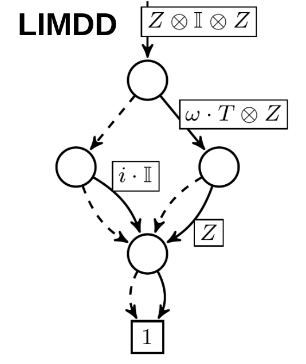
\includegraphics[width=3cm]{limdd}

\end{frame}






